% ====================================================================
%  CHAPTER 3: MATERIALS AND METHODS
%  Write in the future tense for a proposal. Every objective in Chapter 1
%  needs a method here, and nothing here should exceed the scope set in
%  Section 1.7.
% ====================================================================
\chapter{MATERIALS AND METHODS}\label{ch:3}

\section{Research Design}\label{sec:3.1}
\guidance{Name the design, then say how the objectives map onto its stages and what gates progression from one stage to the next.}

{[}Design and analytical sequence.]

\subsection{Overall Workflow}\label{sec:3.1.1}
The work will proceed through the stages shown in Figure~\ref{fig:3.1}.

\begin{figure}[htbp]
  \centering
  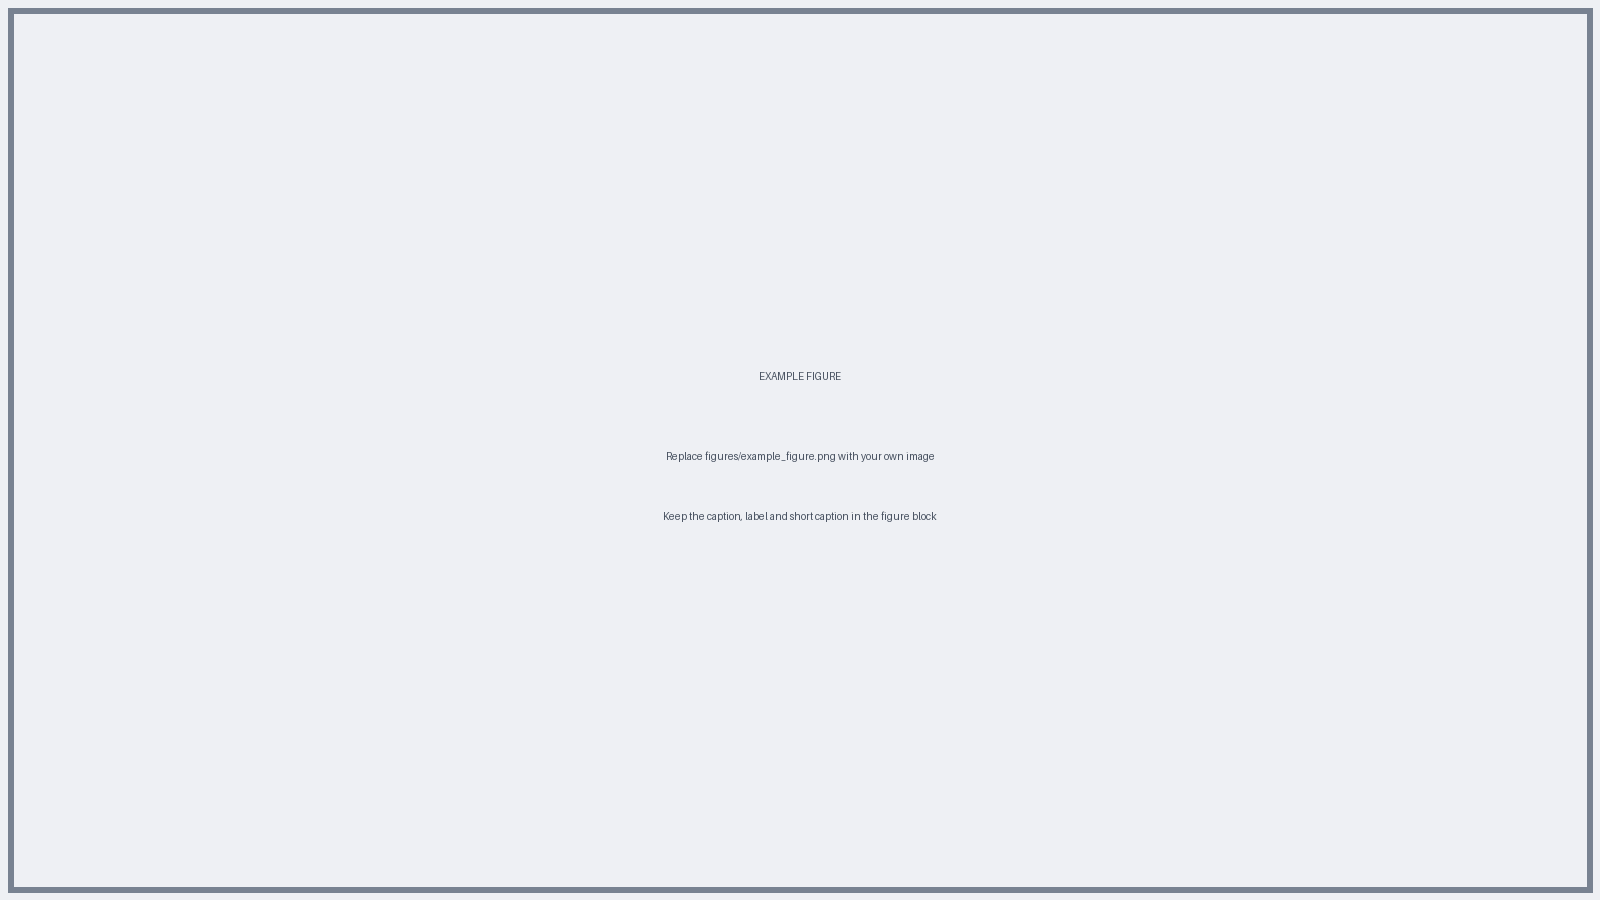
\includegraphics[width=\textwidth]{figures/example_figure.png}
  \caption[Overall study workflow]{Overall study workflow from [first stage] to [final stage]. Source: author.}
  \label{fig:3.1}
\end{figure}

\subsection{Materials, Software and Reproducibility}\label{sec:3.1.2}
\guidance{Record versions. A proposal that names software without versions cannot be reproduced, and examiners notice.}

Table~\ref{tab:3.1} lists the tools to be used.

\begin{table}[htbp]
  \centering
  \caption{Core software, versions and analytical functions.}
  \label{tab:3.1}
  \footnotesize
  \begin{tabularx}{\textwidth}{@{}>{\bfseries}p{0.19\textwidth} X p{0.30\textwidth}@{}}
    \toprule
    Analysis stage & \textbf{Software / version} & \textbf{Primary function} \\
    \midrule
    {[}Stage] & {[}Tool x.y.z] & {[}What it does here] \\
    {[}Stage] & {[}Tool x.y.z] & {[}What it does here] \\
    \bottomrule
  \end{tabularx}
\end{table}

\section{Study Location}\label{sec:3.2}
{[}Where the work will be done, and what facilities that site provides.]

\section{Study Material and Sampling}\label{sec:3.3}

\subsection{Study Material}\label{sec:3.3.1}
{[}Genotypes, accessions, isolates, participants or datasets, with their source and identifiers.]

\subsection{Sampling and Replication}\label{sec:3.3.2}
\guidance{State the experimental unit, the number of independent biological replicates, and what pooling does and does not achieve. Distinguish technical from biological replication.}

{[}Sampling plan, replication and the resulting sample size.]

\subsection{Contingency}\label{sec:3.3.3}
{[}What happens if the material or condition you depend on is not available in time, and the date by which that decision will be taken.]

\section{[Objective 1 Methods]}\label{sec:3.4}
\guidance{One section per objective, with subsections for each procedure. Give thresholds, parameters and acceptance criteria, not just tool names.}

\subsection{[Procedure]}\label{sec:3.4.1}
{[}Method, with parameters, for example an E-value threshold of $1\times10^{-5}$ and coverage of $\geq$~50\%.]

\subsection{[Procedure]}\label{sec:3.4.2}
{[}Method.]

\section{[Objective 2 Methods]}\label{sec:3.5}

\subsection{[Procedure]}\label{sec:3.5.1}
{[}Method.]

\subsection{[Procedure]}\label{sec:3.5.2}
{[}Method.]

\section{Statistical Analysis}\label{sec:3.6}
\guidance{Name the model, the experimental unit, the error control and the reporting convention. Say in advance how assumption failures will be handled, so that the choice is not made after seeing the data.}

{[}Analysis plan, for example: significance at $q<0.05$ after Benjamini-Hochberg correction, with effect sizes and confidence intervals reported alongside adjusted $P$ values.]

\section{Quality Assurance and Quality Control}\label{sec:3.7}
{[}Controls, calibration, exclusion rules, logs and audit trail.]

\section{Ethical and Biosafety Considerations}\label{sec:3.8}
{[}Approvals needed, permissions obtained, waste handling, and a statement of any approvals that fall outside this study.]

\section{Study Limitations and Mitigation}\label{sec:3.9}
Table~\ref{tab:3.2} sets out the anticipated limitations.

\begin{table}[htbp]
  \centering
  \caption{Anticipated limitations, their effects and planned mitigation.}
  \label{tab:3.2}
  \footnotesize
  \begin{tabularx}{\textwidth}{@{}p{0.24\textwidth} p{0.24\textwidth} X@{}}
    \toprule
    \textbf{Limitation} & \textbf{Potential effect} & \textbf{Mitigation} \\
    \midrule
    {[}Limitation] & {[}Effect] & {[}Mitigation] \\
    {[}Limitation] & {[}Effect] & {[}Mitigation] \\
    \bottomrule
  \end{tabularx}
\end{table}

\section{Expected Outputs}\label{sec:3.10}
{[}Datasets, protocols, code, and a statement of what is not an expected output.]

\section{Data Management and Dissemination}\label{sec:3.11}
{[}Storage, backup, identifiers, version control, and how results will be disseminated.]
